\def\slantfrac#1#2{ \hspace{3pt}\!^{#1}\!\!\hspace{1pt}/
  \hspace{2pt}\!\!_{#2}\!\hspace{3pt}
} %Красивые дроби в строчку (например, 1/2)

% \begin{align*}
% f(x) =& x^2\! +3x\! +2 \\
% f(x) =& x^2+3x+2 \\
% f(x) =& x^2\, +3x\, +2 \\
% f(x) =& x^2\: +3x\: +2 \\
% f(x) =& x^2\; +3x\; +2 \\
% f(x) =& x^2\ +3x\ +2 \\
% f(x) =& x^2\quad +3x\quad +2 \\
% f(x) =& x^2\qquad +3x\qquad +2
% \end{align*}

\chapter{Модификация теории Ми для случая многослойной сферы} \label{chapt1}
\section{Современные методы моделирования уравнений Максвелла}
\label{sec:em-methods-intro}
При рассмотрении вопроса о рассеянии и поглощении электромагнитных
волн многослойными сферическими наночастицами в первую очередь
возникает проблема выбора математической модели, которая описывала бы
такую систему.  В настоящее время существует огромное число методов
компьютерного моделирования явлений электромагнетизма достаточно
общего
вида~\cite{Yu-PFDTD-2006,Inan-FDTD-2011,clemson,Bondenson-CEM-2005,Yu-Advanced-FDTD-2011}:
\begin{itemize}
\item метод конечных элементов (finite element method, FEM)
\item метод конечных объёмов во временной области (finite volume
  time-domain, FVTD)
\item метод моментов (method of moments, MoM), обычно реализуемый
  в рамках метода граничных элементов (boundary element method, BEM)
\item метод конечных интегралов (finite integration technique, FIT)
\item метод конечных разностей в временной области (finite difference
  time domain, FDTD)
\item метод конечных разностей в частотной области (finite difference
  frequency domain, FDFD)
\item псевдоспектральный метод во временной области (pseudospectral
  time domain method, PSTD)
\item метод матриц линий передач (transmission line matrix method,
  TLM)
\item приближение дискретных диполей (discrete dipole approximation, DDA)
\end{itemize}
Здесь не упоминаются модификации и усовершенствования этих методов
(иногда существенным образом меняющие исходный алгоритм), как и не
отмечено большое число других методов.  В целом, каждый из методов
можно пытаться классифицировать по следующим параметрам: в основе
лежит интегральная или дифференциальная форма уравнений Максвелла,
метод оперирует данными во временной или в частотной области,
дискретизации подвергается вся модель или только границы её составных
объёмов и т.д.

Сравнение этих методов приводится во многих источниках.
В~\cite{Inan-FDTD-2011} перечисляются такие достоинства FDTD,
как малое время разработки работоспособной программы, его простота
для понимания и то, что он работает с уравнениями Максвелла в явном
виде, не привлекая приёмы линейной алгебры, а также его недостатки:
ступенчатая аппроксимация и большая вычислительная сложность.  При
сравнении FDTD с методом FVTD отмечается, что последний лучше подходит для
неоднородных объектов, время моделирования сопоставимо с временем
FDTD, а основным недостатком является необходимость
дискретизации объёма модели неоднородной сеткой (что в общем случае
является нетривиальной задачей).  Сильные стороны FDFD
демонстрируются в случае, когда необходимо получить установившееся
решение для одной частоты.  Особо ярко это проявляется для материалов,
чья зависимость от частоты не может быть формализована простыми
моделями для FDTD и для систем с высокодобротным резонансом.
Достоинства FEM аналогичны достоинствам  FVTD, а основной
недостаток состоит в том, что необходимо решать всю систему уравнений
(она может быть очень большой) для всего объекта моделирования
сразу. Значимость этого недостатка может быть несколько уменьшена за
счёт использования итеративных методов и ряда других техник, связанных
с предварительными преобразованиями используемых матричных систем
уравнений.  PSTD, относящийся к спектральным методам, характеризуется
тем, что применяет разложение (чаще всего Фурье) полей общего решения
модели.  При этом используется значительно менее плотная сетка
дискретизации, что даёт существенный выигрыш в задействованных памяти
и вычислительных ресурсах компьютера.

В книге~\cite{Bondenson-CEM-2005} для выбранного пространственного
размера задачи (3D) приводится вычислительная сложность разных методов
в зависимости от частоты $f$ изучаемого электромагнитного поля.  Для
FDTD число операций растёт как $O(f^4)$, основной недостаток ---
ступенчатая аппроксимация границ, проходящих под углом к направлениям
прямоугольной сетки дискретизации.  FVTD хорошо справляется со
сложными геометриями объектов модели, требует приблизительно такое же
количество вычислительных ресурсов, что и
FDTD, но обладает слабой <<отложенной>> нестабильностью.
Вычислительная сложность FEM растёт как $O(f^4)$ и для частотной, и
для временной области, он более стабилен, чем FVTD.  Для регулярной 3D
сетки дискретизации TLM может быть представлен в форме, эквивалентной
FDTD.  FIT обладает вычислительной сложностью FDTD, но позволяет
использовать произвольные сетки дискретизации с сохранением
стабильности.  Вычислительная сложность MoM зависит от выбранного
метода решения системы уравнений.  Для fast multipole method (FMM) это
$O(f^3)$, а для multilevel fast multipole algorithm (MLFMA) это
$O(f^2\log f)$.

В книге~\cite{Yu-Advanced-FDTD-2011} на одной и той же аппаратной
платформе производилось моделирование общего набора задач с помощью
коммерчески доступного программного обеспечения~(ПО), основанного на разных
(указанных в скобках) методах: HFSS~(FEM), CST MWS~(FIT), GEMS~(FDTD),
FEKO~(MoM). Сравнение результатов расчётов даёт довольно хорошее
совпадение для CST и GEMS, которые решили весь
набор тестовых задач. GEMS оказался быстрее (иногда в несколько раз)
CST и использовал меньшее количество оперативной памяти.

Объектом изучения настоящей работы является сферическая наночастица,
что позволяет применять специализированные методы. Прежде
всего, это теория Ми для многослойной сферы~\cite{Yang-2003} и её
развитие в виде метода Т-матриц (Multiple Sphere
T-Matrix)~\cite{MacKowski-2012}.  По сравнению с более общими методами
применение этой теории позволяет значительно сократить объём
вычислений, необходимый, например, для расчёта сечений рассеяния и
поглощения.  Дополнительным преимуществом теории Ми является
возможность разделять вклады электрических и магнитных мультиполей в
общий электромагнитный отклик частицы.


\section{Теория Ми для многослойной сферы: расчёт ближнего поля}
\label{sec:Mie}

Более 100 лет назад Густав Ми опубликовал свою оригинальную
работу~\cite{Mie-1908} о взаимодействии плоской электромагнитной волны
с однородной сферой.  Изложенная в ней теория впоследствии получила
его имя и в настоящее время входит в число основных инструментов,
применяемых при анализе задач рассеяния и поглощения сферическими
объектами.  Несмотря на более чем вековую историю теории Ми, работы по
её дальнейшему развитию ведутся и в настоящее время~\cite{Suzuki-2008,
  MacKowski-2012, Lerme-2000, Xu-2005, Li-2006, Gogoi-2010,
  Santiago-2011}.  Довольно часто авторы таких работ предоставляют
доступ к своим программам, реализующим новые разработки в этой
области, что позволяет напрямую сравнивать их между собой.  К
сожалению, большая часть таких программ относится к случаю сферы с
одним или несколькими слоями покрытия. Рядом авторов были предложены
математические модели~\cite{Yang-2003, Pena-scattnlay-2009},
позволяющие изучать многослойные сферы с произвольным числом
слоёв~\cite{Sheehan-2013,Selmke-2012}.  Основная сложность при этом
связана с численной реализацией этих моделей.

Рассмотрим рассеяние плоской волны, поляризованной вдоль
координаты~$x$, следуя классическому подходу, изложенному в книге
К.Ф.~Борена и Д.Р.~Хафмена~\cite{Bohren-1983}.  В сферических
координатах такую волну можно записать как:
\begin{equation*}
  \label{eq:bh4.21}
  {\rmfamily \mathbf{E}}_i = E_0 e^{i{\rmfamily k}r\cos\theta}
  {\boldsymbol{\hat{\mathbf{\rmfamily e}}}}_{x}\:,
\end{equation*}
\begin{equation*}
{\boldsymbol{\hat{\mathbf{\rmfamily e}}}}_{x} = \,\sin\theta\, \cos\phi\, 
{\boldsymbol{\hat{\mathbf{\rmfamily e}}}}_{r} 
+\, \cos\theta\, \sin \phi\, {\boldsymbol{\hat{\mathbf{\rmfamily e}}}}_{\theta}
-\, \sin \phi\, {\boldsymbol{\hat{\mathbf{\rmfamily e}}}}_{\phi}\:,
\end{equation*}
где $E_0$ амплитуда падающего поля, а $r,\,\theta,\,\phi$ и
${\boldsymbol{\hat{\mathbf{\rmfamily e}}}}$ --- полярные координаты и единичный вектор для
выбранной системы координат, $k$ волновой вектор падающей волны.
Тогда решение для рассеянного поля выражается в виде разложения в ряд:
\begin{align}
  \label{eq:vector-harm1}
{\rmfamily \mathbf{E}}_s &=\sum_{n=1}^{\infty} E_n \left( i a_n {\rmfamily
    \mathbf{N}}_{e1n}^{(3)} - b_n{\rmfamily\mathbf{M}_{o1n}^{(3)}} \right)\:,\\
  \label{eq:vector-harm2}
{\rmfamily \mathbf{H}}_s &=\frac{k}{\omega\mu}
 \sum_{n=1}^{\infty} E_n \left( i b_n {\rmfamily
    \mathbf{N}}_{o1n}^{(3)} + a_n{\rmfamily\mathbf{M}_{e1n}^{(3)}} \right)\:,  
\end{align}
где $E_n=i^nE_0(2n+1)/n(n+1)$, $n$ порядок мультиполя, $E_0$ амплитуда
падающего поля, $a_n$ и $b_n$ коэффициенты разложения, соответствующие
электрическим и магнитным мультиполям,
${\rmfamily \mathbf{N}}_{e1n}^{(j)}$,
${\rmfamily \mathbf{N}}_{o1n}^{(j)}$,
${\rmfamily\mathbf{M}_{o1n}^{(j)}}$ и
${\rmfamily\mathbf{M}_{e1n}^{(j)}}$ сферические векторные гармоники
\footnote{см.~далее уравнения (\labelcref{eq:2p1,eq:2p2,eq:2p3,eq:2p4})
и (\labelcref{eq:2p1mod,eq:2p2mod,eq:2p3mod,eq:2p4mod})}, обычно
выражающиеся через тригонометрические функции, полиномы Лежандра и
сферические функции Бесселя и Ханкеля, $\omega$ частота падающей
волны, $\mu$ магнитная проницаемость в вакууме.  Аналогичным образом
может быть выражено поле внутри $l$-ого слоя стратифицированной
сферы~\cite{Yang-2003}:
\begin{align}
{\rmfamily \mathbf{E}}_l &=\sum_{n=1}^{\infty} E_n \left(
                     c_n^{(l)}{\rmfamily\mathbf{M}}_{o1n}^{(1)}
                     -i d_n^{(l)} {\rmfamily \mathbf{N}}_{e1n}^{(1)}
                     +i a_n^{(l)} {\rmfamily \mathbf{N}}_{e1n}^{(3)}
                     - b_n^{(l)}{\rmfamily\mathbf{M}}_{o1n}^{(3)} 
                     \right)\label{eq:3p1}\:,\\
{\rmfamily \mathbf{H}}_l &=\frac{k_l}{\omega\mu} \sum_{n=1}^{\infty} E_n
                     \left(
                      d_n^{(l)}{\rmfamily\mathbf{M}}_{e1n}^{(1)} 
                     +i c_n^{(l)} {\rmfamily \mathbf{N}}_{o1n}^{(1)} 
                     -i b_n^{(l)} {\rmfamily \mathbf{N}}_{o1n}^{(3)} 
                     - a_n^{(l)}{\rmfamily\mathbf{M}}_{e1n}^{(3)} 
                     \right)\:,\label{eq:3p2}  
\end{align}
где для каждого слоя определены коэффициенты разложения $d_n^{(l)}$ и
$c_n^{(l)}$ электрического и магнитного поля для входящей волны
(направленной к центру частицы) и, аналогично, $a_n^{(l)}$ и
$b_n^{(l)}$ для исходящей волны.  Связь между всеми коэффициентами
разложения можно выразить в виде системы рекуррентных уравнений,
которые получаются из граничных условий на непрерывность
нормальных компонент полей на границе между слоями~\cite{Yang-2003}:

\begin{equation} % \tag{S} % tag - вписывает свой текст
  \label{eq:A2d1}
    % \begin{multlined}
    \begin{alignedat}{2}
d^{(l+1)}_{n}m_{l} \psi^{\prime}_{n}&{\left (m_{l+1} x_{l} \right )}
- a^{(l+1)}_{n} m_{l} \zeta^{\prime}_{n}{\left (m_{l+1} x_{l} \right )}-\\
& - d^{(l)}_{n} m_{l+1} \psi^{\prime}_{n}{\left (m_{l} x_{l} \right )} 
+ a^{(l)}_{n} m_{l+1} \zeta^{\prime}_{n}{\left (m_{l} x_{l} \right )}
= 0\:,
\end{alignedat}
\end{equation}
\begin{equation} % \tag{S} % tag - вписывает свой текст
  \label{eq:A2d2}
\begin{alignedat}{2}
c^{(l+1)}_{n} m_{l} \psi_{n}&{\left (m_{l+1} x_{l} \right )}
  - b^{(l+1)}_{n} m_{l} \zeta_{n}{\left (m_{l+1} x_{l} \right )}-\\
&- c^{(l)}_{n} m_{l+1} \psi_{n}{\left (m_{l} x_{l} \right )} 
+b^{(l)}_{n} m_{l+1} \zeta_{n}{\left (m_{l} x_{l} \right )}  =0\:,
\end{alignedat}
\end{equation}
\begin{equation} % \tag{S} % tag - вписывает свой текст
  \label{eq:A2d3}
\begin{alignedat}{2}
c^{(l+1)}_{n} \psi^{\prime}_{n}&{\left (m_{l+1} x_{l} \right )}
- b^{(l+1)}_{n} \zeta^{\prime}_{n}{\left (m_{l+1} x_{l} \right )}-\\
&- c^{(l)}_{n} \psi^{\prime}_{n}{\left (m_{l} x_{l} \right )} 
+b^{(l)}_{n} \zeta^{\prime}_{n}{\left (m_{l} x_{l} \right )}   =0\:,
\end{alignedat}
\end{equation}
\begin{equation} % \tag{S} % tag - вписывает свой текст
  \label{eq:A2d4}
\begin{alignedat}{2}
 d^{(l+1)}_{n} \psi_{n}&{\left (m_{l+1} x_{l} \right )}
- a^{(l+1)}_{n} \zeta_{n}{\left (m_{l+1} x_{l} \right )}-\\
& - d^{(l)}_{n} \psi_{n}{\left (m_{l} x_{l} \right )} 
+ a^{(l)}_{n} \zeta_{n}{\left (m_{l} x_{l} \right )}   =0\:,
\end{alignedat}
% \end{multlined}
\end{equation}
где $m_l$ показатель преломления в слое, нормированный на показатель
преломления окружающего пространства, $x_l=kr_l$ параметр размера
внешнего радиуса слоя, выраженный через его радиус,
$\psi_{n}(z) = z j_n(z)$ и $\zeta_{n}(z) = z h_n^1(z)$ функции
Риккати-Бесселя, выраженные через сферические функции Бесселя и
Ханкеля.  Из выражений для падающей и рассеянной волны получаются
дополнительные условия на коэффициенты разложения
$c_n^{(L+1)}=d_n^{(L+1)}=1$, $a_n^{(L+1)}=a_n$ и $b_n^{(L+1)}=b_n$,
где $L$ общее число слоёв. Так как у центрального слоя $l=1$ нет
внутренней границы, то $a_n^{(1)}=b_n^{(1)}=0$. Последнее условие
является избыточным для системы
уравнений~(\labelcref{eq:A2d1,eq:A2d2,eq:A2d3,eq:A2d4}), и поэтому оно
было использовано для дополнительной проверки самосогласованности
работы компьютерной программы.  Система
уравнений~(\labelcref{eq:A2d1,eq:A2d2,eq:A2d3,eq:A2d4}) распадается на
две независимых линейных системы и может быть решена явно. После
проведения необходимых алгебраических преобразований были получены
значения коэффициентов разложения в виде обратной рекуррентной
последовательности:
\begin{equation}
\label{eq:6p1}
a^{(l)}_n = \frac
{
    {D^{(1)}_{n}}{\left (m_{l} x_{l} \right )}
    T_1\left (m_{l+1} x_{l} \right )
    +
    T_3\left (m_{l+1} x_{l} \right )
    m_{l}/m_{l+1}
}
{
   \zeta_{n}\left (m_{l} x_{l} \right )
   U\left (m_{l} x_{l} \right )
}\:,
\end{equation}
\begin{equation}
\label{eq:6p2}
b^{(l)}_n = \frac
{
    {D^{(1)}_{n}}{\left (m_{l} x_{l} \right )}
    T_2\left (m_{l+1} x_{l} \right )
    m_{l}/m_{l+1}
    +
    T_4\left (m_{l+1} x_{l} \right )
}
{
   \zeta_{n}\left (m_{l} x_{l} \right )
   U\left (m_{l} x_{l} \right )
}\:,
\end{equation}
\begin{equation}
\label{eq:6p3}
c^{(l)}_n = \frac
{
    {D^{(3)}_{n}}{\left (m_{l} x_{l} \right )}
    T_2\left (m_{l+1} x_{l} \right )
    m_{l}/m_{l+1}
    +
    T_4\left (m_{l+1} x_{l} \right )
}
{
   \psi_{n}\left (m_{l} x_{l} \right )
   U\left (m_{l} x_{l} \right )
}\:,
\end{equation}
\begin{equation}
\label{eq:6p4}
d^{(l)}_n = \frac
{
    {D^{(3)}_{n}}{\left (m_{l} x_{l} \right )}
    T_1\left (m_{l+1} x_{l} \right )
    +
    T_3\left (m_{l+1} x_{l} \right )
    m_{l}/m_{l+1}
}
{
   \psi_{n}\left (m_{l} x_{l} \right )
   U\left (m_{l} x_{l} \right )
}\:,
\end{equation}
используя
\begin{equation*}
  U(z) =    {D^{(1)}_{n}}(z) - {D^{(3)}_{n}}(z)\:,
\end{equation*}
\begin{equation*}
  T_1(z) =   a^{(l+1)}_{n}  \zeta_{n}(z) 
           - d^{(l+1)}_{n}  \psi_{n}(z)\:,
\end{equation*}
\begin{equation*}
  T_2(z) =   b^{(l+1)}_{n}  \zeta_{n}(z) 
           - c^{(l+1)}_{n}  \psi_{n}(z)\:,
\end{equation*}
\begin{equation*}
  T_3(z) =  d^{(l+1)}_{n}  D^{(1)}_{n}(z)  \psi_{n}(z) 
          - a^{(l+1)}_{n}  D^{(3)}_{n}(z)  \zeta_{n} (z)\:,
\end{equation*}
\begin{equation*}
  T_4(z) =  c^{(l+1)}_{n}  D^{(1)}_{n}(z)  \psi_{n}(z) 
          - b^{(l+1)}_{n}  D^{(3)}_{n}(z)  \zeta_{n} (z)\:,
\end{equation*}
где $D^{(1)}_{n} = \psi^{\prime}_{n}/\psi_{n}$ и
$D^{(3)}_{n} = \zeta^{\prime}_{n}/\zeta_{n}$ логарифмические
производные функций Риккати-Бесселя. Подставляя
(\labelcref{eq:6p1,eq:6p2,eq:6p3,eq:6p4}) в уравнения (\ref{eq:3p1}) и
(\ref{eq:3p2}), можно вычислить величину электрического и магнитного
поля внутри и снаружи многослойной сферы. Это является основным
результатом настоящей главы.

С очевидностью, решение системы
уравнений~(\labelcref{eq:A2d1,eq:A2d2,eq:A2d3,eq:A2d4}) может быть
выражено и в виде прямой рекуррентной последовательности. Такое решение было
получено, но после реализации в компьютерной программе проявилась
его плохая численная устойчивость, поэтому в настоящей работе
оно не используется.

При этом возникает дополнительная сложность, связанная с вычислением
сферических векторных гармоник, выражаемых через сферические функции
Бесселя ($j=1$) и Ханкеля ($j=3$) первого рода $z_n^{(j)}$~\cite{Bohren-1983}:
\begin{equation}
  \label{eq:2p1}
 \begin{alignedat}{2}
  {\rmfamily\mathbf{M}}_{o1n}^{(j)} =\cos \phi\,
         \pi_n\!\left(\cos \theta\right)
         z_n^{(j)}\!\left( \rho \right)\,
         {\boldsymbol{\hat{\mathbf{\rmfamily e}}}}_{\theta}   
-\,\sin \phi\,
         \tau_n\!\left(\cos \theta\right)
         z_n^{(j)}\!\left( \rho \right)\,
         &{\boldsymbol{\hat{\mathbf{\rmfamily e}}}}_{\phi}\:,
 \end{alignedat}
\end{equation}
%
\begin{equation}
  \label{eq:2p2}
 \begin{alignedat}{2}
  {\rmfamily\mathbf{M}}_{e1n}^{(j)} =-\,\sin \phi\,
         \pi_n\!\left(\cos \theta\right)
         z_n^{(j)}\!\left( \rho \right)\,
         {\boldsymbol{\hat{\mathbf{\rmfamily e}}}}_{\theta}   
-\, \cos \phi\,
         \tau_n\!\left(\cos \theta\right)
         z_n^{(j)}\!\left( \rho \right)\,
         &{\boldsymbol{\hat{\mathbf{\rmfamily e}}}}_{\phi}\:,
 \end{alignedat}
\end{equation}
%
\begin{equation}
  \label{eq:2p3}
 \begin{alignedat}{2}
{\mathbf{N}}_{o1n}^{(j)} = \,{\sin} \phi\,n\!\left(n+1\right)
         {\sin}\theta\,
         \pi_n\!\left({\cos} \theta\right)
         \frac{
               z_n^{(j)}\!\left( \rho \right)
              }{\rho}\,
           &{\boldsymbol{\hat{\mathbf{\mathrm e}}}}_{r}\,+   \\
+\,
{\sin} \phi\,
         \tau_n\!\left({\cos} \theta\right)
         \frac{
            \left[\rho z_n^{(j)}\!\left( \rho \right)\right]^{\prime}
              }{\rho}\,
            &{\boldsymbol{\hat{\mathbf{\mathrm e}}}}_{\theta}\,+   \\
+\,
{\cos} \phi\,
         \pi_n\!\left({\cos} \theta\right)
         \frac{
            \left[\rho z_n^{(j)}\!\left( \rho \right)\right]^{\prime}
              }{\rho}\,
            &{\boldsymbol{\hat{\mathbf{\rmfamily e}}}}_{\phi}\:,
\end{alignedat}
\end{equation}
%
\begin{equation}
  \label{eq:2p4}
 \begin{alignedat}{2}
{\rmfamily \mathbf{N}}_{e1n}^{(j)} = \,\cos \phi\,n\!\left(n+1\right)
         \sin\theta\,
         \pi_n\!\left(\cos \theta\right)
         \frac{
               z_n^{(j)}\!\left( \rho \right)
              }{\rho}\,
           &{\boldsymbol{\hat{\mathbf{\rmfamily e}}}}_{r} \,+  \\
+\,
\cos \phi\,
         \tau_n\!\left(\cos \theta\right)
         \frac{
            \left[\rho z_n^{(j)}\!\left( \rho \right)\right]^{\prime}
              }{\rho}\,
            &{\boldsymbol{\hat{\mathbf{\rmfamily e}}}}_{\theta} \,+  \\
+\,
\sin \phi\,
         \pi_n\!\left(\cos \theta\right)
         \frac{
            \left[\rho z_n^{(j)}\!\left( \rho \right)\right]^{\prime}
              }{\rho}\,
            &{\boldsymbol{\hat{\mathbf{\rmfamily e}}}}_{\phi}\:,
\end{alignedat}
\end{equation}
где обезразмеренное расстояние до центра сферы $\rho=kr$, а угловые
функции
\begin{equation*}
  \label{eq:bh4.46}
  \pi_n=\frac{P_n^1}{\cos\theta} \qquad \mbox{и} \qquad \tau_n = \frac{dP_n^1}{d\theta}
\end{equation*}
выражены через функцию Лежандра $P_n^m$, которая
задаётся через производную полинома Лежандра $P_n$ в виде
\begin{equation*}
  \label{eq:bh4.25}
  P_n^m\left(\mu\right)=\left(1-\mu^2\right)^{m/2}\frac{d^{\,m}P_n(\mu)}{d\mu^m}\:,
\end{equation*}
где $\mu = \cos\theta$. Чтобы рассчитать значения угловых функций,
необходимо воспользоваться рекуррентными
соотношениями~\cite{Wiscombe-1980}
\begin{equation}
  \label{eq:bh4.47a}
  \pi_0 = 0, \qquad \pi_1 = 1, \qquad
  \pi_n = \frac{2n-1}{n-1}\cos\theta\,\pi_{n-1} - \frac{n}{n-1}\pi_{n-2}\:,
\end{equation}
\begin{equation}
  \label{eq:bh4.47b}
  \tau_n = n\cos\theta\,\pi_{n} + (n+1)\pi_{n-1}\:,
\end{equation}
доказавшими свою численную устойчивость.  Таким образом, основную
сложность при вычислении значений сферических векторных гармоник
представляет суммирование рядов, выражающих сферические функции
Бесселя.  Плохая сходимость таких рядов особенно заметна в случае
комплексного аргумента с большой мнимой частью.  Для решения этой
проблемы в настоящей главе предлагается следующий вид сферических
векторных гармоник:
\begin{equation}
  \label{eq:2p1mod}
 \begin{alignedat}{2}
  {\rmfamily\mathbf{M}}_{o1n}^{(j)} =\cos \phi\,
         \pi_n\!\left(\cos \theta\right)
         \frac{r_n^{(j)}\!\left( \rho \right)}{\rho}\,
         {\boldsymbol{\hat{\mathbf{\rmfamily e}}}}_{\theta}   
-\,\sin \phi\,
         \tau_n\!\left(\cos \theta\right)
         \frac{r_n^{(j)}\!\left( \rho \right)}{\rho}\,
         &{\boldsymbol{\hat{\mathbf{\rmfamily e}}}}_{\phi}\:,
 \end{alignedat}
\end{equation}
%
\begin{equation}
  \label{eq:2p2mod}
 \begin{alignedat}{2}
  {\rmfamily\mathbf{M}}_{e1n}^{(j)} =-\,\sin \phi\,
         \pi_n\!\left(\cos \theta\right)
         \frac{r_n^{(j)}\!\left( \rho \right)}{\rho}\,
         {\boldsymbol{\hat{\mathbf{\rmfamily e}}}}_{\theta}   
-\, \cos \phi\,
         \tau_n\!\left(\cos \theta\right)
         \frac{r_n^{(j)}\!\left( \rho \right)}{\rho}\,
         &{\boldsymbol{\hat{\mathbf{\rmfamily e}}}}_{\phi}\:,
 \end{alignedat}
\end{equation}
%
\begin{equation}
  \label{eq:2p3mod}
 \begin{alignedat}{2}
{\rmfamily \mathbf{N}}_{o1n}^{(j)} = \,\sin \phi\,n\!\left(n+1\right)
         \sin\theta\,
         \pi_n\!\left(\cos \theta\right)
         \frac{
           r_n^{(j)}\!\left( \rho \right)
              }{\rho^2}\,
           &{\boldsymbol{\hat{\mathbf{\rmfamily e}}}}_{r}\,+   \\
+\,
\sin \phi\,
         \tau_n\!\left(\cos \theta\right)
         \frac{
           D_n^{(j)}\!(\rho) r_n^{(j)}\!(\rho)
              }{\rho}\,
            &{\boldsymbol{\hat{\mathbf{\rmfamily e}}}}_{\theta}\,+   \\
+\,
\cos \phi\,
         \pi_n\!\left(\cos \theta\right)
         \frac{
           D_n^{(j)}\!(\rho) r_n^{(j)}\!(\rho)
              }{\rho}\,
            &{\boldsymbol{\hat{\mathbf{\rmfamily e}}}}_{\phi}\:,
\end{alignedat}
\end{equation}
%
\begin{equation}
 \label{eq:2p4mod}
 \begin{alignedat}{2}
{\rmfamily \mathbf{N}}_{e1n}^{(j)} = \,\cos \phi\,n\!\left(n+1\right)
         \sin\theta\,
         \pi_n\!\left(\cos \theta\right)
         \frac{
               r_n^{(j)}\!\left( \rho^2 \right)
              }{\rho}\,
           &{\boldsymbol{\hat{\mathbf{\rmfamily e}}}}_{r}\,+   \\
+\,
\cos \phi\,
         \tau_n\!\left(\cos \theta\right)
         \frac{
           D_n^{(j)}\!(\rho) r_n^{(j)}\!(\rho)
              }{\rho}\,
            &{\boldsymbol{\hat{\mathbf{\rmfamily e}}}}_{\theta}\,+   \\
+\,
\sin \phi\,
         \pi_n\!\left(\cos \theta\right)
         \frac{
           D_n^{(j)}\!(\rho) r_n^{(j)}\!(\rho)
              }{\rho}\,
            &{\boldsymbol{\hat{\mathbf{\rmfamily e}}}}_{\phi}\:,
\end{alignedat}
\end{equation}
где используются функции Риккати-Бесселя $r_n^{(1)} = \psi_n$ и
$r_n^{(3)} = \zeta_n$ и их логарифмические производные, благодаря чему
автору удалось заметно увеличить численную устойчивость расчёта по
теории Ми. Дело в том, что функции Риккати-Бесселя могут быть записаны
в виде обратной рекуррентный последовательности с хорошей сходимостью
для более широкого диапазона
аргументов~\cite{Wiscombe-1980,Mackowski-1990} по сравнению со
сферическими функциями Бесселя следующим образом:
\begin{equation*}
  \label{eq:pena16a}
  D_{N_{\scalebox{0.65}{\rmfamily max}}}^{(1)}(z) = 0 + i0\:,
\end{equation*}
\begin{equation*}
  \label{eq:pena16b}
  D_{n-1}^{(1)}(z) = \frac{n}{z} -\frac{1}{D_n^{(1)}(z)+n/z}\:,\quad n=N_{\max}, \ldots, 0\:,
\end{equation*}
где выражение для количества членов рекурсии $N_{\rmfamily nmax}$ было
предложено в работе~\cite{Wiscombe-1980}:
\begin{equation*}
  N_{\max} = \max\left(N_{\rmfamily stop}, \left|m_lx_l\right|,
    \left|m_lx_{l-1}\right|
\right) + 15\:, \quad l=1,2,\ldots,L\:,
\end{equation*}
\begin{equation*}
\label{eq:pena17}
  N_{\rmfamily stop}=
\begin{cases}
x_L+4x_L^{\slantfrac{1}{3}}+1\:,\quad & 0.02\leqslant x_L<8\:,\\
x_L+4.05x_L^{\slantfrac{1}{3}}+2\:,\quad & 8\leqslant x_L<4\,200\:,\\
x_L+4x_L^{\slantfrac{1}{3}}+2\:,\quad & 4\,200\leqslant x_L<20\,000\:.\\
\end{cases}
\end{equation*}
В работе~\cite{Mackowski-1990} была показана численная устойчивость
следующего метода для вычисления $D_n^{(3)}$:
\begin{equation*}
  \label{eq:pena18a}
  \psi_0(z)\zeta_0(z)=\frac{1}{2}
\left[
1-(\cos\,2a+i\,\sin\,2a)exp(-2b)
\right],
\end{equation*}
\begin{equation*}
  \label{eq:pena18b}
D_0^{(3)} = i\:,
\end{equation*}
\begin{equation*}
  \label{eq:pena18c}
  \psi_n(z)\zeta_n(z)=   \psi_{n-1}(z)\zeta_{n-1}(z)
\left[
\frac{n}{z}-D_{n-1}^{(1)}(z)
\right]
\left[
\frac{n}{z}-D_{n-1}^{(1)}(z)
\right],
\end{equation*}
\begin{equation*}
  \label{eq:pena18d}
D_n^{(3)}(z) = D_n^{(1)}(z)+\frac{i}{\psi_n(z)\zeta_n(z)}\:,\quad
n=1,\ldots, N_{\max}\:,
\end{equation*}
где $z=a+ib$. Функции Риккати-Бесселя задаются следующими
выражениями~\cite{Wiscombe-1980,Mackowski-1990}:
\begin{equation*}
  \label{eq:pena20a}
  \psi_0(z) = \sin(z)\:,
\end{equation*}
\begin{equation*}
  \label{eq:pena20b}
\psi_n(z) = \psi_{n-1}(z)
\left[
\frac{n}{z}-D_{n-1}^{(1)}(z)
\right], \quad n=1,\ldots, N_{\max}\:,
\end{equation*}
\begin{equation*}
  \label{eq:pena21a}
\zeta_0(z) = \sin(z) - i\,\cos(z)\:,
\end{equation*}
\begin{equation*}
  \label{eq:pena21b}
\zeta_n(z) = \zeta_{n-1}(z)
\left[
\frac{n}{z}-D_{n-1}^{(3)}(z)
\right], \quad n=1,\ldots, N_{\max}\:.
\end{equation*}
Таким образом, в настоящем разделе предложен математический аппарат,
позволяющий вычислять локальные поля в случае падения плоской
электромагнитной волны на сферическую многослойную
частицу. Разработанный метод отличается высокой надёжностью и
устойчивостью в широком диапазоне входных параметров, что, среди
прочих факторов, вызвано использованием оригинального вида сферических
векторных гармоник в представлении через логарифмические производные
функций Риккати-Бесселя.


\section{Компьютерная реализация алгоритма расчёта по теории Ми}
\label{sec:code}

% \subsection{Выбор алгоритма, языка программирования, оптимизация
% быстродействия}

Для проведения расчётов с использованием выражений, полученных в
разделе~\ref{sec:Mie}, наиболее рациональным является применение
компьютера.  Для этого необходимо разработать новую или модифицировать
ранее созданную компьютерную программу. Второй вариант, как менее
трудоёмкий, является предпочтительным.  При этом необходимо принимать
во внимание целый ряд факторов:
\begin{itemize}
\item Функциональность уже готовых программ.
\item Возможности по их модификации, которые прежде всего определяются
  доступностью исходного текста программы и используемыми языками
  программирования.
\item Количество и качество документации, описывающее работу
  программы, наличие возможности получить консультацию у авторов,
  простота её использования.
\item Производительность.
\end{itemize}

В сети Интернет~\cite{scattport,wiki-mie-codes} и в
литературе~\cite{Wriedt-2009} можно найти описания десятков программ,
выполняющих расчёты по теории Ми.  Довольно часто они базируются на
коде BHMIE, описанном в книге К.Ф.~Борена и
Д.Р.~Хафмена~\cite{Bohren-1983}.  Заслуженное признание получил код
MIEV0~\cite{Wiscombe-1980}, основанный на специальном
алгоритме~\cite{Lentz-76} для представления сферических функций
Бесселя. Дальнейшее развитие метода дало возможность моделировать
агрегаты из нескольких сферических частиц~\cite{Mackowski-96,Xu-95}.

Ряд работ описывает взаимодействие света с многослойной
сферой~\cite{Kai-94,Wu-97, Bhandari-85}.  Наибольшей численной
устойчивостью, насколько об этом можно судить из обзора литературы,
обладает алгоритм, предложенный в 2003 году W.~Yang~\cite{Yang-2003} и
реализованный O.~Pe\~{n}a-Rodr\'{i}guez в 2009
году~\cite{Pena-scattnlay-2009} в виде публично доступной программы.
Именно эта реализация и была выбрана в качестве основы для программы,
разрабатываемой в рамках настоящей диссертации, как наиболее полно
соответствующая изложенным выше требованиям.  Тем не менее, для
достижения цели, поставленной в диссертации, оказалась необходима
существенная переработка исходной программы.

Прежде всего это касалось ряда технических моментов. Так как программа
была написана на языке программирования Си, то в ней использовалось
прямое выделение памяти для хранения данных.  Применение
родственного языка Си\texttt{++} позволило перейти к использованию
динамических массивов, что заметно упростило
программу и сделало более эффективной её эксплуатацию в качестве
внешней библиотеки.

Использование объектно-ориентированной парадигмы программирования
позволило автоматизировать ряд рутинных операций, тем самым избавив
конечного пользователя от их выполнения, сохранив при этом достаточно
чёткую структуру программы.  Прежде всего это касается проверки
корректности вводимых параметров модели (толщины слоёв должны быть
положительными, для каждого слоя требуется задать толщину и показатель
преломления, было реализовано большое число прочих проверок). Кроме
того, появилась возможность задания параметров модели в размерных
величинах, а перевод в безразмерные величины происходит внутри
программы. Всё это уменьшает возможность ошибок из-за человеческого
фактора.

Следующий момент связан с выполнением операций над комплексными
числами.  В оригинальной программе для выполнения арифметических
действий (умножения, деления, вычитания и так далее) определялись
явные функции вида \verb+Cmul(a,b)+, \verb+Cdiv(a,b)+,
\verb+Csub(a,b)+, где \verb+a+ и \verb+b+ переменные, содержащие
значение комплексного числа.  Переход на использование языка
программирования Си\texttt{++} позволил воспользоваться возможностями
стандартной библиотеки \verb+std::complex+, а запись упомянутых
арифметических операций приобрела естественный вид, например,
\verb!a*b!, \verb!a/b!, \verb!a-b! и тому подобное.  Это значительно
упрощает ввод в текст вычислительной программы выражений, полученных
при аналитическом анализе проблемы.

Важной характеристикой работы любой программы является её
быстродействие, в этом случае существенное значение оказывает выбор
языка программирования.  С момента своего появления (вторая половина
1950-х) и вплоть до начала 2000-х годов лучшим языком для научных и
инженерных вычислений было принято считать Фортран, специально для
этих целей и разработанный. Весомым плюсом языка является наличие
огромного количества свободно распространяющихся библиотек
математических операций. В то же время достаточно широкое
распространение получил язык Си, став одним из самых используемых
языков программирования, а также заложив основу синтаксиса для других
языков (например, Си\texttt{++}).  К недостаткам Си можно было отнести
лишь недостаточно высокую производительность, из-за чего аналоги
программ на Фортране были быстрее вплоть до десятка
раз~\cite{Veldhuizen-1997}. Тем не менее, улучшение оптимизации кода
компиляторами Cи/Cи\texttt{++}, рост числа специализированных
библиотек, популяризация языков Си и Си\texttt{++}, связанная с
распространением операционной системы Unix (и с сопутствующим ростом
количества доступных качественных учебных материалов по языку и
специальной литературы, приведшей, как следствие, к увеличению числа
высококвалифицированных специалистов, использующих эти языки для
решения широкого спектра задач), позволили значительно повысить среднюю
эффективность вычислительных программ на языках Си и Си\texttt{++},
достигнув паритета с аналогичными программами на
Фортране~\cite{Veldhuizen-1997,Markovich-FDTD-2013}.  Это означает,
что дальнейший рост быстродействия ограничен аппаратными возможностями
компьютера.  Кроме того, к преимуществам языков Си и Си\texttt{++}
относится значительно меньшая стоимость разработки и развития сложных
проектов.  Всё вместе это позволяет сделать вывод о том, что в
настоящее время Си\texttt{++} является наилучшим выбором языка для
программирования требовательных к вычислениям задач.

Само по себе написание программы на наиболее подходящем для конечной
задачи языке программирования не гарантирует достижения наилучшего
быстродействия.  Стандартной процедурой для увеличения быстродействия
является временн\'ое профилирование программы, которое позволяет
выявить места, требующие больше всего вычислительных ресурсов.  Далее
оптимизация производится только для подобных мест, так как остальные
части программы не оказывают существенного влияния на общее время
выполнения.  При доработке настоящей программы было выявлено несколько
таких мест, среди которых особо хотелось отметить вычисление
уравнений~\ref{eq:bh4.47a} и~\ref{eq:bh4.47b}.  Для них наиболее
трудоёмкой частью с вычислительной точки зрения них оказалась задача
нахождения косинуса угла. Так как значение угла не меняется внутри
цикла рекурсии, то предварительное вычисление вне цикла дало большую
часть ускорения работы программы для ряда тестовых примеров.

В итоге программа для проведения вычислений по теории Ми была полностью
переработана, она получила возможность расчёта полей, оптимизация уже
существовавших алгоритмических решений позволила сократить время
выполнения в 2.2 раза.  Все описанные доработки были с благодарностью
приняты оригинальным автором программы Ovidio Pe\~{n}a-Rodr\'{i}guez и
в полном объёме добавлены в исходной код
программы~\cite{Scattnlay-web}.

Предложенное представление сферических векторных гармоник через
логарифмические производные функций Риккати-Бесселя позволило
значительно расширить границы численной устойчивости метода.  Для
дальнейшего развития программы расчёта начаты работы по использованию
библиотек контролируемой точности вычислений (arbitrary-precision
arithmetic).  Первые результаты на этом пути показали практическую
реализуемость подобного решения.

% \subsection{Верификация работы на тестовых примерах}

Важным этапом работ была верификация программы на нескольких
тестовых примерах:
\begin{itemize}
\item Однородная сфера, что является предельным случаем многослойной
  сферы с одним слоем $L=1$.
\item Сфера с покрытием $L=2$. Этот и предыдущий примеры позволяют
  провести сравнения с хорошо изученными случаями, для которых
  известно аналитическое решение.
\item Трёхслойная наночастица $Si/Ag/Si$. В этом случае сравнение
  будет проводиться с результатами полноволнового моделирования
  методом FDTD, которое выполнялось с использованием коммерческого ПО.
\item Многослойное маскирующее покрытие, сравнение выполняется с
  коммерческим ПО CST MWS, использующим для моделирования в частотной
  области метод конечных элементов.
\end{itemize}

В качестве первого теста был взят пример из работы М.В.~Башевого
и~др.~\cite{Bashevoy-2005}, в которой рассматривалось образование
нановихрей в наночастице золота. 
\begin{figure}[p]
  \begin{minipage}[ht]{0.99\linewidth}
    \centering{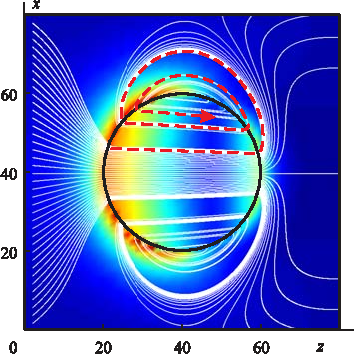
\includegraphics[width=0.59\linewidth]{bashevoj-oe-13-21-8372-fig}}
  \end{minipage}\\
  \vfill
  \begin{minipage}[ht]{0.99\linewidth}
    \centering{а)}
  \end{minipage}\\
  \vfill
  \begin{minipage}[ht]{0.99\linewidth}
    \centering{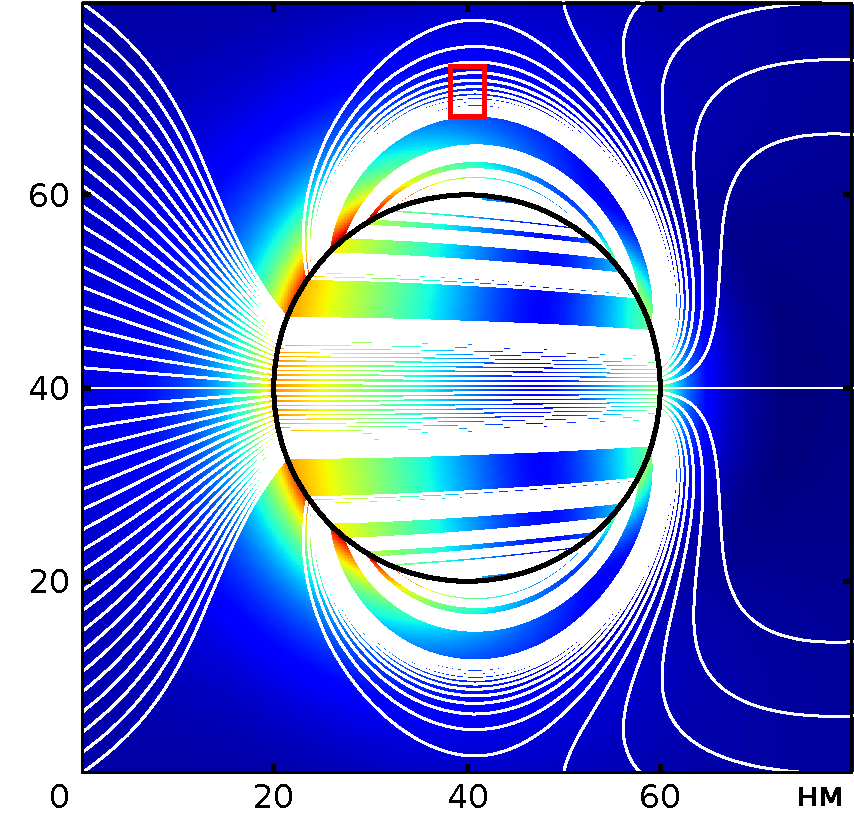
\includegraphics[width=0.59\linewidth]{bulk-Ag-flow-R20-XZ-Pabs-mark3}
    }
  \end{minipage}\\
  \begin{minipage}[ht]{0.99\linewidth}
    \centering{б)}
  \end{minipage}
  \caption{Золотая сфера $r=20$~нм при облучении светом с длиной волны
    $\lambda=354$~нм, (a) результат из работы М.В.~Башевого
    и~др.~\cite{Bashevoy-2005}, (б) результат расчёта ближнего поля по
    выражениям из раздела~\ref{sec:Mie}. Цвет меняется от синего к
    красному что характеризует рост величины вектора Пойнтинга, касательная к
    белым линиям --- его направление. Волна падает слева
    направо.\label{img:vortex}}
\end{figure}
Расчёт полей при этом проводился с помощью метода конечных элементов в
программе Comsol~\cite{Comsol-web}. Так как дискретизация модели производится с помощью
неупорядоченной сетки, то нарушается собственная симметрия системы,
что хорошо видно на перепечатанном из оригинальной работы
рисунке~\ref{img:vortex}(а).  В области больших значений амплитуды
вектора Пойнтинга в верхней половине на границе сферы амплитуда
меняется достаточно плавно, а в нижней наблюдается несколько областей
с локальными максимумами.

На рисунке~\ref{img:vortex}(б) его верхняя и нижняя половины
зеркально-симметричны, как и стоит ожидать от аналитического
расчёта. В целом стоит отметить хорошее совпадение результатов
полноволнового моделирования в коммерческом ПО с результатами,
полученными в настоящей главе.  Кроме уже отмеченных небольших различий
в амплитуде вектора Пойнтинга заметны и сопутствующие различия в
линиях потока энергии. В работе М.В.~Башевого
и~др.~\cite{Bashevoy-2005} указано, что эти линии были получены в
результате численного решения уравнения
\begin{equation*}
  \frac{d\mathbf{\rmfamily A}}{dt}=\mathbf{\rmfamily S}(\mathbf{\rmfamily A})\:,
\end{equation*}
где $\,\mathbf{\rmfamily A}(t)$ поле вектора Пойнтинга
$\,\mathbf{\rmfamily S}=\left[\mathbf{\rmfamily
    E}\times\mathbf{\rmfamily H}\right]$, $\,t$ ---~координата вдоль
линии.  При таком подходе положение линий потока энергии может быть
дополнительно искажено из-за ошибок в расчёте поля
$\mathbf{\rmfamily A}$. Это становится особенно заметно в структурах с
резкими изменениями амплитуды поля, например, на границе сферы, или
при наличии вихрей потока энергии, где протяжённость этих линий
значительно увеличивается.

Для того чтобы увеличить точность построения, в настоящей работе был
предложен следующий алгоритм, который позволяет контролировать
возникающую ошибку. Линия потока энергии строится из некой начальной
точки, как упорядоченная последовательность прямых отрезков, где
каждый последующий начинается в конце предыдущего. Направление
отрезка задаётся вещественной частью среднего значения за период
колебаний вектора Пойнтинга
\begin{equation*}
  \left\langle\mathbf{\rmfamily S}\right\rangle = \frac{1}{2}
  \left[\mathbf{\rmfamily E}\times\mathbf{\rmfamily H}^*\right]\:.
\end{equation*}
Длина текущего отрезка зависит от направления вектора
$\operatorname{\mathbb{R}e}\left\langle\mathbf{\rmfamily S}\right\rangle$ в
его конечной точке. Если его направление отличается от текущего
на значение большее, чем пороговый угол (эта величина является
параметром построения и в настоящей работе, если не указано иное, была
принята равной одному градусу), то длина отрезка уменьшается в два
раза, и расчёт производится заново до тех пор, пока не будет найдено
удовлетворительное значение длины. Перед расчётом
следующего отрезка используемая длина увеличивается в два раза, что
позволяет быстро достичь максимально возможного значения для
заданной точности построения.

При прохождении через границу раздела двух сред непрерывной является
только нормальная компонента вектора Пойнтинга. Поэтому, если отрезок
пересекает эту границу, то уменьшение его длины практически не влияет
на направление следующего отрезка. Чтобы избежать бесконечного
уменьшения длины в такой ситуации, был задан второй параметр
построения ---~минимальная длина отрезка.  В настоящей работе, если не
указано иное, это значение бралось в $2\,000$ раз меньше радиуса
внутреннего слоя многослойной сферы, что позволяет с контролируемой
точностью совмещать изломы линии потока энергии с границами
раздела. При этом значительно сокращается необходимый объём вычислений
для построения областей с небольшой кривизной линий потока энергии.

Результат работы предложенного алгоритма для построения линий потока
энергии можно оценить на рисунке~\ref{img:vortex}(б).  По сравнению с
рисунком~\ref{img:vortex}(а) внутри и вблизи частицы удалось получить
более плавное изменение расстояния между линиями потока энергии,
стартовые точки для которых были расположены через равные интервалы на
некотором отдалении от рассматриваемой сферы.  Уменьшая значение параметров
построения (пороговый угол и минимальная длина отрезка), несложно
проверить его стабильность.
\begin{figure}[t] {\centering
  \begin{minipage}[ht]{0.49\linewidth}        
    \centering{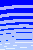
\includegraphics[width=0.6\linewidth]{bulk-Ag-flow-R20-XZ-Pabs-crop} }
  \end{minipage}
  \begin{minipage}[ht]{0.49\linewidth}
    \centering{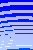
\includegraphics[width=0.6\linewidth]{bulk-Ag-flow-R20-XZ-Pabs-fine-crop} }
  \end{minipage}
}\\
{\centering
  \begin{minipage}[ht]{0.49\linewidth}
    \centering{а)}
  \end{minipage}
  \begin{minipage}[ht]{0.49\linewidth}
    \centering{б)}
  \end{minipage}
}
\caption{Фрагмент из области на рисунке~\ref{img:vortex}(б),
  выделенный красным прямоугольником. Случай (а) исходных параметров
  для построения линий потока энергии, (б) пороговый угол уменьшен в 2
  раза, минимальная длина отрезка в 10 раз.\label{img:vortex-crop}}
\end{figure}
Для этого на рисунке~\ref{img:vortex-crop}(а) было построено
увеличенное изображение фрагмента рисунка~\ref{img:vortex}(б) из
области, выделенной красным прямоугольником. На
рисунке~\ref{img:vortex-crop}(б) были изменены параметры построения
линий потока энергии: пороговый угол уменьшен в 2 раза, минимальная
длина отрезка уменьшена в 10 раз. Видно, что хотя общий характер
картины не изменился, тем не менее есть несколько отличий. Все линии
немного сместились (приблизительно на ширину изображаемой линии),
более важное изменение касается расстояния между ними. На
рисунке~\ref{img:vortex-crop}(а) оно убывает неравномерно, например,
для нижних четырёх линий расстояние между парой вторая/третья
больше, чем между парами линий первая/вторая и третья/четвёртая. У
такого поведения нет физического обоснования, оно вызвано небольшой
ошибкой при построении линий потока энергии.  После изменения
параметров построения в сторону обеспечения большей точности ситуация
исправилась, визуально расстояние между линиями на
рисунке~\ref{img:vortex}(б) изменяется монотонно при их последовательном
переборе по вертикали.
 
Для сравнения случая двухслойных структур была выбрана программа
BHFIELD~\cite{Suzuki-2008,Suzuki-2013}, доступная в
сети Интернет.  Это позволило задавать идентичные параметры
моделирования для BHFIELD и программы, разработанной в настоящей
главе. Моделировалась диэлектрическая частица с радиусом $R_1=50$~нм и
показателем преломления $n_1=1.53413$, покрытая 10~нм слоем серебра (в
результате внешний радиус частицы $R_2=60$~нм) с показателем
преломления $n_2=0.565838+i7.23262$ (что соответствует длине волны
$\lambda = 1\,064$~нм), расположенная в диэлектрической матрице с
показателем преломления $n_m=1.3205$.  Результаты, полученные в версии
BHFIELD для двойной точности вычислений, полностью соответствуют
результатам программы, разработанной в настоящей главе.

Случай сферы, состоящей из трёх слоёв, проверялся с использованием
коммерческого пакета моделирования Lumerical
FDTD~\cite{Lumerical-web}. Рассматривалась система $Si/Ag/Si$ с
радиусами $r_l=\{17.74, 41.05, 64\}$~нм, длина волны падающего
излучения $\lambda = 800$~нм, при этом относительная диэлектрическая
проницаемость бралась равной $\varepsilon_{Si} = 13.64 + i 0.047$ для
кремния и $\varepsilon_{Ag} = -28.05 + i 1.525$ для серебра.
Результаты расчёта методом FDTD и по теории Ми представлены на
рисунке~\ref{img:fdtd}.
\begin{figure}[p] 
  \begin{minipage}[ht]{0.99\linewidth}
    \centering{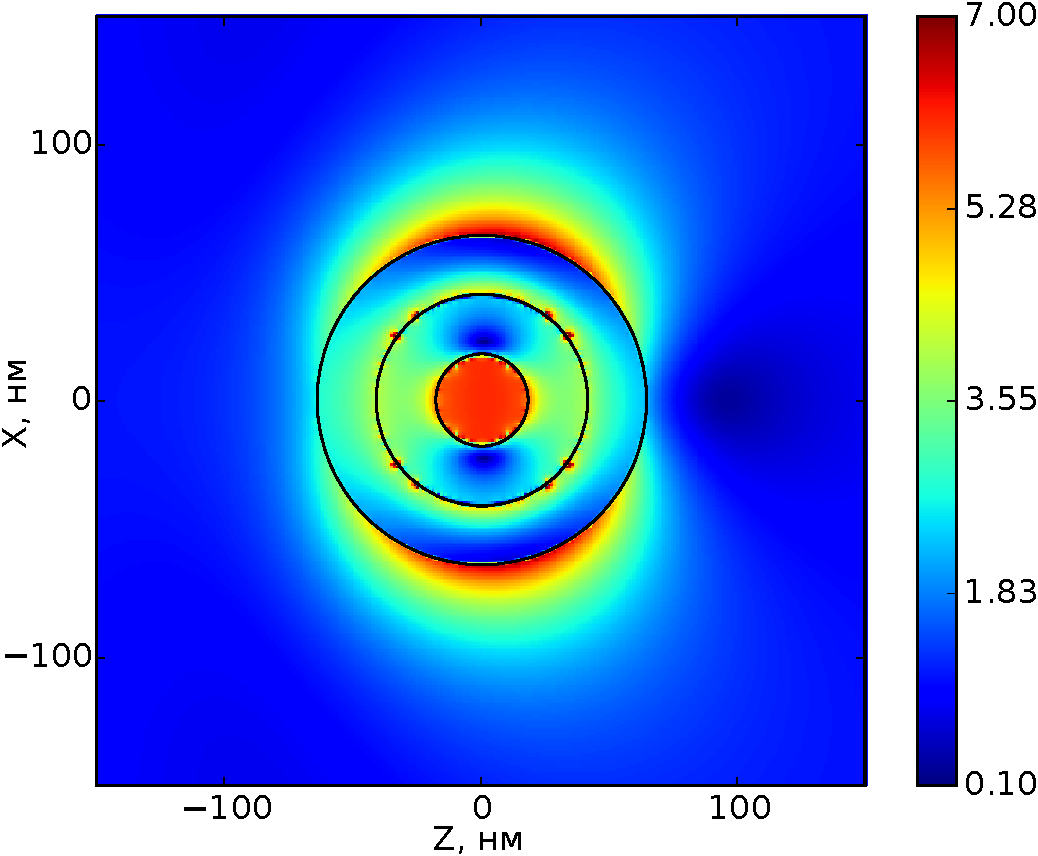
\includegraphics[width=0.67\linewidth]{lumerical-R64-XZ-Eabs}}
  \end{minipage}\\
  \vfill
  \begin{minipage}[ht]{0.99\linewidth}
    \centering{а)}
  \end{minipage}\\
  \vfill
  \begin{minipage}[ht]{0.99\linewidth}
    \centering{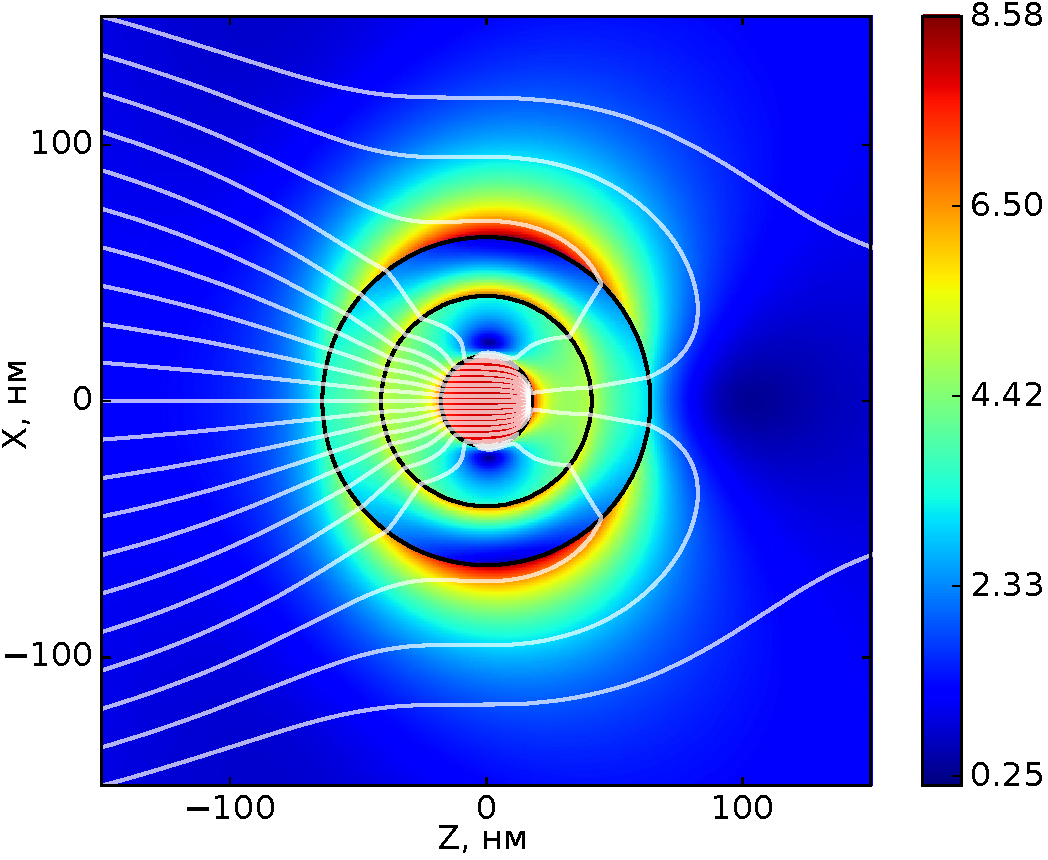
\includegraphics[width=0.67\linewidth]{SiAgSi-absorber-flow-R64-XZ-Eabs}
    }
  \end{minipage}\\
  \vfill
  \begin{minipage}[ht]{0.99\linewidth}
    \centering{б)}
  \end{minipage}
  \caption{Картина ближнего поля для частицы $Si/Ag/Si$ с общим
    радиусом 64~нм. (a) Результат моделирования в Lumerical FDTD, (б)
    результат расчёта ближнего поля по выражениям из
    раздела~\ref{sec:Mie}. Цвет характеризует величину электрического
    поля $|E|/|E_0|$, касательная к белым линиям --- направление
    вектора Пойнтинга. Волна падает слева направо.\label{img:fdtd}}
\end{figure}

В целом картина ближнего поля в обоих случаях оказалась довольно
похожа: для сечения в плоскости поляризации электрическое поле внутри
частицы сконцентрировано в центральной части. Тем не менее,
наблюдается ряд различий, связанных со спецификой FDTD.

В первую очередь необходимо отметить, что для расчёта методом FDTD
вначале производится дискретизация модели с помощью прямоугольной
сетки. Качество расчёта сильно зависит от размера ячейки в этой сетке,
для трёхмерной модели при уменьшении длины ребра ячейки в 2 раза
количество необходимой оперативной памяти компьютера увеличивается в 8
раз.  Общее время расчёта при этом возрастает в 16 раз, так как, кроме
возросшего количества данных, используемых для модели, дополнительно в
2 раза приходится уменьшать шаг по времени (это необходимо для
обеспечения численной устойчивости модели, что определяется критерием
Куранта-Фридрихса-Леви~\cite{Courant-1941}). Другими словами, для
того чтобы обеспечить одинаковый период эволюции по часам модели,
приходится в 2~раза увеличить количество вычислений с данными одной
ячейки.

Такой резкий рост вычислительной сложности с уменьшением шага
дискретизации существенно ограничивает достижимую точность
моделирования методом FDTD. Для получения картины поля на
рисунке~\ref{img:fdtd}а потребовалось около 2-х часов работы мощного
стационарного компьютера при полной загрузке шести ядер центрального
процессора, в то время как расчёт по теории Ми для
рисунка~\ref{img:fdtd}б занял около двух минут при загрузке одного
ядра.

Другая проблема использования прямоугольной сетки заключается в том,
что приходится применять ступенчатую аппроксимацию гладких
поверхностей в пространстве модели (исключение составляют куски
плоскости, ориентированные вдоль граней ячейки дискретизации). В
случае рассмотрения резонансных структур, это приводит к существенным
ошибкам в вычислении поля на границе раздела между слоями, которая не
может быть убрана даже за счёт использования очень мелкого шага
дискретизации.  Для частичного решения этой проблемы в Lumerical FDTD
применяется конформное сопряжение, тем не менее в случае, когда
граница раздела проходит достаточно близко к узлу сетки дискретизации
могут возникать численные резонансы. Восемь таких резонансов, попарно
расположенные на границе между внешним и средним слоем покрытия,
хорошо видны на рисунке~\ref{img:fdtd}а. При небольшом изменении
шага дискретизации эти резонансы исчезнут (но могут появиться новые в
других местах).

Следующее различие, которое можно обнаружить при сравнении, связано с
амплитудой электрического поля.  Расчёт методом FDTD даёт меньшее
значение в центре частицы по сравнению с теорией Ми (приблизительно на
30\%).  Это может быть связано с двумя особенностями расчёта FDTD.

Во-первых, для моделирования рассеяния на частице, расположенной в
бесконечной среде, используется граничное условие в виде идеально
поглощающего слоя (perfectly matched layer, PML). Так как отражение от
такой границы практически отсутствует, то распределение поля перед ней
с хорошей степенью точности совпадает со случаем
<<открытых>> граничных условий, который тождественен бесконечной среде.
Однако формализм PML прежде всего относится с случаю
распространяющихся волн, а в ситуации ближнего поля, когда размеры
объекта оказываются сопоставимы с длиной волны, подобное поведение
может исказить картину поля. Это можно довольно просто понять на
примере вихрей, представленных на рисунке~\ref{img:vortex}.  В
случае свободного пространства поток энергии отдаляется на некоторое
расстояние от частицы и возвращается без потерь. Если на его пути
разместить слой поглощающего вещества, то часть энергии не вернётся в
частицу, что приведёт к уменьшению плотности энергии и связанной с ней
напряжённостью электромагнитного поля.  Таким образом,
необходимым условием для корректности расчёта при использовании
 PML является достаточно большое расстояние между
моделируемой частицей и границей. В рассматриваемом случае оно было
задано равным приблизительно длине волны, так как размер частицы много
меньше, то большую часть моделируемого объёма занимает пустое
пространство. Таким образом, дальнейшее увеличение этого отступа,
например, в 2 раза, приведёт к увеличению объёма модели в 8
раз. Проведение такого расчёта оказалось технически не реализуемым на
применявшихся компьютерах.

Во-вторых, так как расчёт методом FDTD ведётся во временной области,
то моделируется падение на систему и дальнейшее взаимодействие с ней
широкополосного электромагнитного импульса.  Моделирование
прекращается в тот момент, когда практически вся энергия импульса
будет либо рассеяна объектом, либо поглощена.  Чтобы получить величину
поля для какой-то одной длины волны, в точке наблюдения записывается
зависимость напряжённости поля от времени, после чего производится
дискретное преобразование Фурье этого сигнала. Для построения
картины распределения поля на выбранной частоте используется
соответствующая амплитуда в каждой ячейке моделирования в
плоскости рисунка. Таким образом и было построено изображение для
рисунка~\ref{img:fdtd}а. Проблема может возникнуть при наличии
собственных резонансов в модели, что относится и к нашему случаю, где
частота падающей волны приходится на максимум дипольного отклика
частицы. Так как во временной области подаваемый импульс содержит
всего несколько периодов колебания, то этого может оказаться
недостаточно, чтобы в полной мере выявить резонансные свойства
системы.  Это можно исправить, используя более узкую полосу входного
сигнала, что будет соответствовать большему количеству колебаний.
Увеличение числа колебаний потребует пропорционального
увеличения времени расчёта, что ограничивает возможности метода FDTD
по изучению систем с высокодобротным резонансом. Указанные особенности
позволяют сделать вывод о хорошем соответствии результатов, полученных
двумя разными методами расчёта.


Последний пример, выбранный для сравнения, является наиболее сложным
как с точки зрения расчёта по теории Ми, так и для любого
полноволнового метода. Сфера из идеального электрического проводника
(perfect electric conductor, PEC) диаметром $1.5\lambda$ находится
внутри многослойного (32 слоя) покрытия толщиной около
$0.21\lambda$. Свойства таких покрытий будут подробно рассмотрены в
главе~\ref{chapt3}, где на рисунке~\ref{img:designs}б представлена
структура используемого покрытия.
\begin{figure}[p] 
  \begin{minipage}[ht]{0.95\linewidth}
    \centering{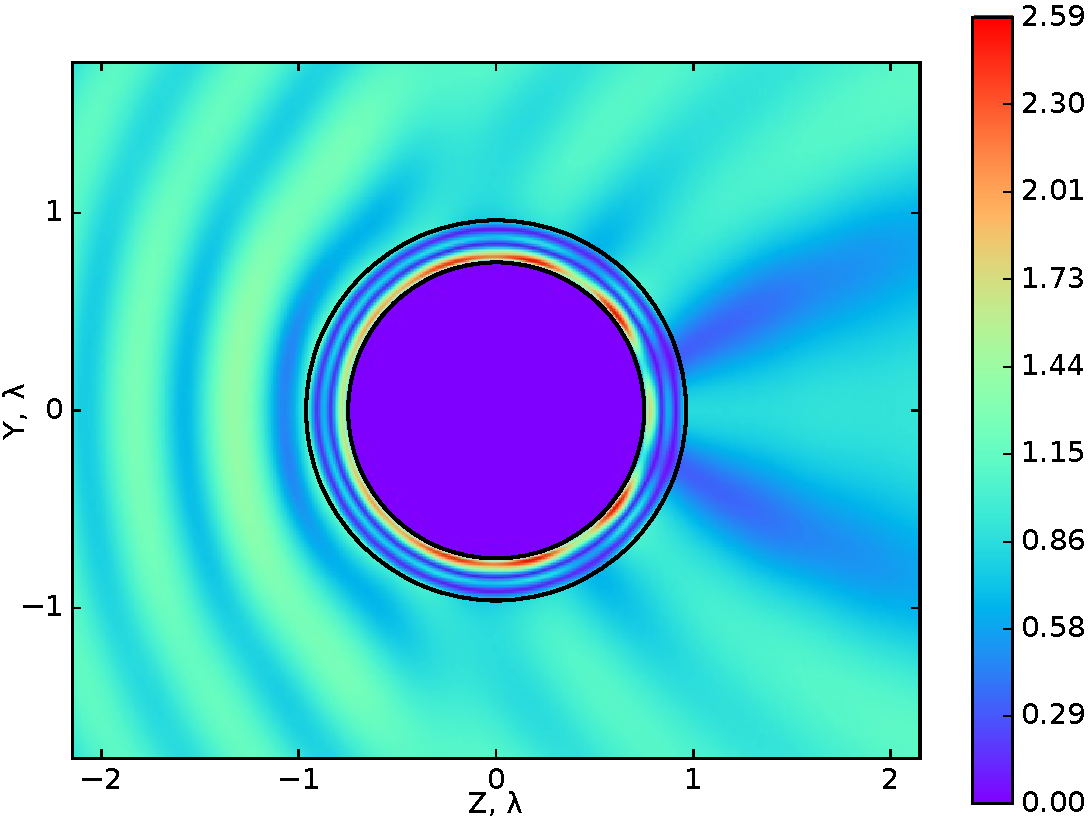
\includegraphics[width=0.79\linewidth]{SiAgSi-absorber-flow-CST-XZ-Eabs}}
  \end{minipage}\\
  \vfill
  \begin{minipage}[ht]{0.99\linewidth}
    \centering{а)}
  \end{minipage}\\
  \vfill
  \begin{minipage}[ht]{0.95\linewidth}
    \centering{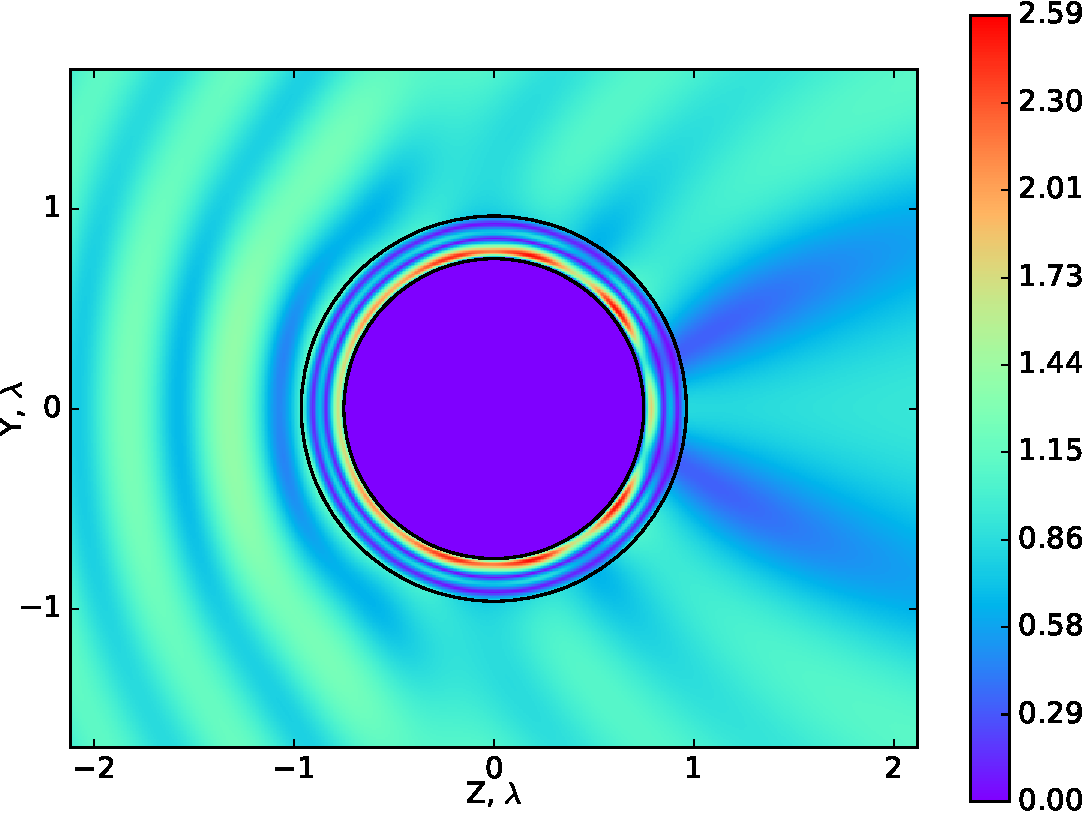
\includegraphics[width=0.79\linewidth]{PEC-index-dv-R4-YZ-Eabs}}
  \end{minipage}\\
  \vfill
  \begin{minipage}[ht]{0.99\linewidth}
    \centering{б)}
  \end{minipage}
  \caption{32-слойное диэлектрическое маскирующее покрытие вокруг
    сферы из идеального электрического проводника. (a) результат
    моделирования в CST MWS с помощью FEM в частотной области, (б)
    результат расчёта ближнего поля по выражениям из
    раздела~\ref{sec:Mie}. Цвет характеризует величину электрического
    поля $|E|/|E_0|$. Волна падает слева направо.\label{img:e32layer}}
\end{figure}

Моделирование с помощью CST~\cite{CST-web} производилось в частотном
пространстве с использованием метода конечных элементов. Дискретизация
модели проводилась нерегулярной тетрагональной сеткой, общее число
элементов разбиения составило около 4 миллионов.  С целью уменьшения
объёма моделирования использовались плоскости симметрии, имеющиеся в
модели. Было выбрано открытое граничное условие с заданным уровнем
отражения -40~dB. Моделирование при этом продолжалось приблизительно
сутки, что существенно отличается от случая с использованием теории
Ми, где для той же системы расчёт занял около 5 минут.

В данном случае совпадение результатов моделирования оказалось очень
хорошим, различие между двумя методами расчёта составило менее 0.4\%
для величины полного сечения рассеяния, значение TSCS составило
$1.809\lambda^2$ и $1.802\lambda^2$ при моделировании с помощью CST и
используя теорию Ми соответственно.  Картины ближнего поля оказались
весьма похожи, как по форме распределения, так и по величине.

\section{Выводы}

В главе рассмотрены различные методы теоретического исследования
взаимодействия электромагнитного поля и многослойной сферической
наночастицы. Лучше всего для этого подходит теория Ми, для расчёта был
выбран алгоритм с максимальной численной устойчивостью.  Были получены
явные рекуррентные соотношения для коэффициентов Ми внутри
многослойной сферы, выраженные через логарифмические производные
функций Риккати-Бесселя в виде обратной последовательности.  Эти
соотношения были добавлены в компьютерную программу, выполняющую
вычисления в рамках задачи Ми. Корректность полученных выражений и
работы модифицированной программы была проверена на ряде примеров с
использованием результатов разных авторов, а также других численных и
аналитических методов.



% ссылки на собственные работы:~\cite{vakbib1, confbib1}
% Сошлёмся на приложения: Приложение \ref{AppendixA}, Приложение \ref{AppendixB2}.
% Сошлёмся на формулу: формула \eqref{eq:equation1}.
% Сошлёмся на изображение: рисунок \ref{img:knuth}.

% Используя команду \verb|\labelcref| из пакета \verb|cleveref|, можно
% красиво ссылаться сразу на несколько формул
% (\labelcref{eq:equation1,eq:equation3,eq:equation2}), даже перепутав
% порядок ссылок \verb|(\labelcref{eq:equation1,eq:equation3,eq:equation2})|.
\clearpage